\begin{figure}[h]
    \centering
    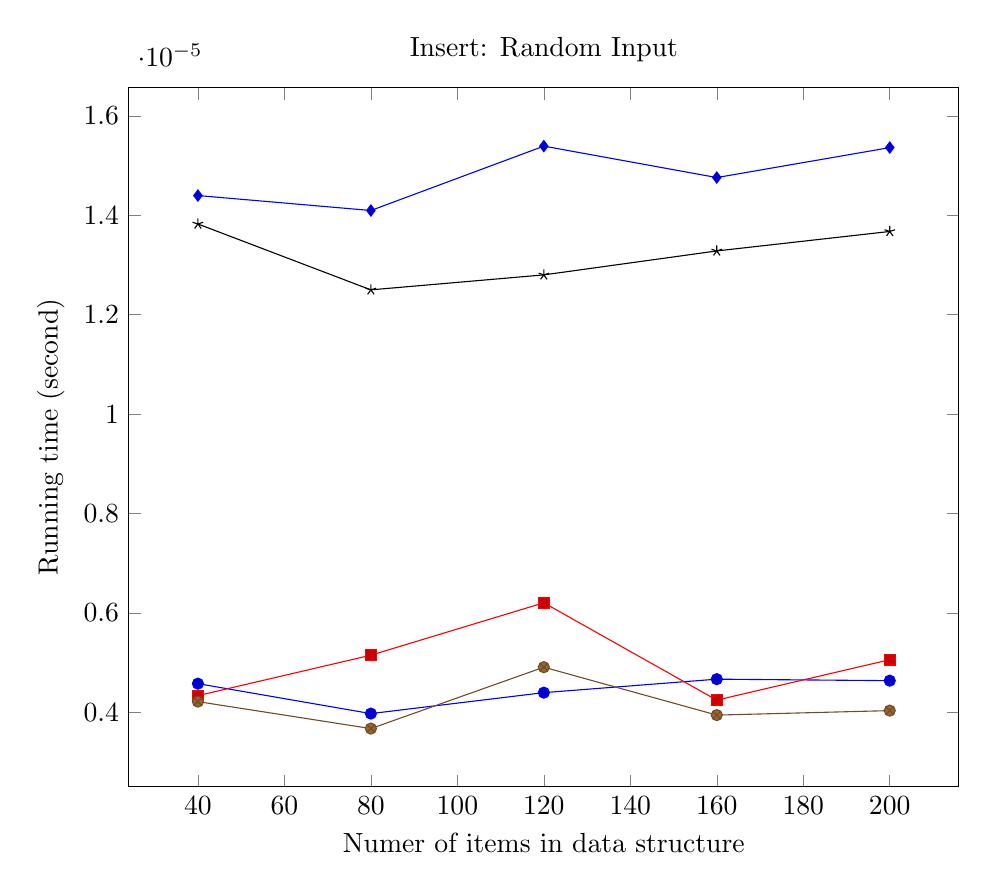
\begin{tikzpicture}
        \begin{axis}[
            xlabel={Numer of items in data structure},
            ylabel={Running time (second)},
            title={Insert: Random Input},
            width=\textwidth
        ]
		\addplot coordinates {
			(200, 4.638100185871963e-06)
			(160, 4.668217719938639e-06)
			(120, 4.397159916535997e-06)
			(80, 3.975514445286877e-06)
			(40, 4.577865118449153e-06)
		};
		\addplot coordinates {
			(200, 5.059745657476355e-06)
			(160, 4.246572247978974e-06)
			(120, 6.204211937088644e-06)
			(80, 5.150098258255298e-06)
			(40, 4.336924849113189e-06)
		};
		\addplot coordinates {
			(200, 4.035749512354414e-06)
			(160, 3.9453969115754715e-06)
			(120, 4.909157989274604e-06)
			(80, 3.674339108528102e-06)
			(40, 4.216454714622841e-06)
		};
		\addplot coordinates {
			(200, 1.3673360288635195e-05)
			(160, 1.3281832350742206e-05)
			(120, 1.2799951812070275e-05)
			(80, 1.249877647495623e-05)
			(40, 1.3823947956836945e-05)
		};
		\addplot coordinates {
			(200, 1.5359942174342223e-05)
			(160, 1.4757591500824674e-05)
			(120, 1.5390059708053626e-05)
			(80, 1.4095005759884316e-05)
			(40, 1.439618109664309e-05)
		};
        \legend{}
        \end{axis}
    \end{tikzpicture}
    \caption{Average of 0 operations, benchmarked every 0, starting at 0.}
\end{figure}